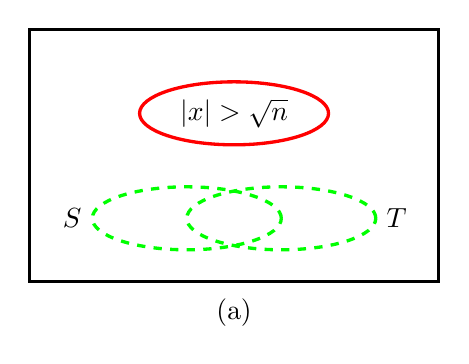
\begin{tikzpicture}[scale=0.80]
%Style macros
\tikzset{ST/.style={green, dashed, very thick}}
\tikzset{myset/.style={red, very thick}}
\tikzset{square/.style={black, very thick}}

%Circle macro, for rx and ry diameters
\tikzset{rx/.style={x radius=#1},ry/.style={y radius=#1}}

%Macros for graph parameters (length/height/radii)
\pgfmathsetmacro{\length}{6.5}
\pgfmathsetmacro{\height}{4}
\pgfmathsetmacro{\rad}{(\length-0.5)/4}
\pgfmathsetmacro{\rx}{2}
\pgfmathsetmacro{\ry}{5}

%Define array for labels
\def\lab{{"a","b","c", "d"}}

%Low left corners at (0,0), (0,-height-2), (length+2,0), (length+2, -height-2)
\def\xcoords{{0, \length+1,		    0,  \length+1}}
\def\ycoords{{0, 		 0,-\height-1, -\height-1}}

%%% MAIN CODE %%%

%Draw constant stuff (rectangles + sets S,T)
\foreach \i in {1} 
{ 

	\pgfmathsetmacro{\labelz}{\lab[\i-1]}
	\pgfmathsetmacro{\x}{\xcoords[\i-1]}
	\pgfmathsetmacro{\y}{\ycoords[\i-1]}

	%Draw rectangle, label at (length/2, \y-0.5)
	\draw[square] (\x, \y) rectangle (\x + \length,\y + \height) node[] at (\x + \length/2,\y - 0.5){(\labelz)};
	
	%Draw sets S and T
	\draw[ST] (\x + \rad + 1,\y + 1) circle [rx=\rad cm, ry=0.5cm] node[black, left=1.2cm]{$S$};
	\draw[ST] (\x + \length - \rad -1,\y + 1) circle [rx=\rad cm, ry=0.5cm] node[black, right=1.2cm]{$T$};

}

%Draw custom stuff for each rectangle
%Rectangle a
\pgfmathsetmacro{\x}{\xcoords[0]}
\pgfmathsetmacro{\y}{\ycoords[0]}
\draw[myset] (\x + \length/2, \y+\height-\height/3) circle[rx = \rad cm, ry = 0.5cm] node[black]{$|x|> \sqrt{n}$};
\node[red] at (\x+0.9*\length, \y + 0.9*\height) {\Huge \xmark};

\end{tikzpicture}
